\documentclass[11pt]{article}		% Précise le type de document, et la taille de la police de caractère
\usepackage[margin=2.5cm]{geometry} % Précise les marges du document
\usepackage{amsmath,amsthm,amssymb,amsfonts}	% Pour pouvoir inclure certains symboles et environnements mathématiques
\usepackage[french]{babel}	% Pour préciser la langue du document
\usepackage{graphicx}	% Pour inclure des images
\usepackage{color}	% Pour inclure du texte en couleur
\usepackage{units}	% Pour pouvoir tapper les unités correctement
\usepackage{pgf,tikz}	% Utilisation du module tikz, qui permet de tracer des belles images
\usetikzlibrary{arrows} % Quand on exporte une image GeoGebra, on a besoin de préciser cela
\usepackage{hyperref}	% Pour include des liens dans le document
\usepackage[T1]{fontenc}	% Précise la façon dont le document actuel est encodé
\usepackage[utf8]{inputenc}	% Précise comment le texte est saisi : cela permet de tapper directement les accents
\newcommand{\N}{\mathbb{N}}	% Commande personnelle, plus rapide pour tapper les ensembles
\newcommand{\Z}{\mathbb{Z}}	% Commande personnelle, plus rapide pour tapper les ensembles
\newcommand{\R}{\mathbb{R}}	% Commande personnelle, plus rapide pour tapper les ensembles
\usepackage{cprotect}	% Pour pouvoir personaliser la légende des figures
 
\begin{document}
\thispagestyle{empty}	% Pour éviter d'avoir un en-tête et un pied de page sur la page couverture

\includegraphics[width=5cm]{logo.jpg}	% Pour inclure le logo (on précise la largeur de l'image)
\vspace{4cm}	% Espacement vertical
\begin{center}	% On centre le texte
{\huge \bf Travail Pratique 2}\\	% \huge fait que le texte est gros, \bf fait que le texte est gras
\vspace{3cm}
\large Travail présenté à Philippe Giguère dans le cadre du cours \emph{GLO-7021 : Introduction à la robotique mobile}\\
\vspace{3cm}
Travail réalisé par NAOUSSI SIJOU, Wilfried Armand \\
NI: 536 773 538
\vfill	% On va jusqu'au bas de la page avant de mettre le texte ci-dessous
Hiver 2022
\end{center}

% ========================= Filtre de Kalman Linéaire  ========================= 
\newpage
\section {Filtre de Kalman linéaire : estimation de la température d'un échantillon}

\subsection{a) Valeurs de $\Phi$, $\Gamma$, $\Lambda$}

\noindent Variable d'état:  X = [x], où x est la température de l'échantillon \\
\noindent Variable de commande: u = [-1.6] \\

\noindent X(k+1) = X(k) - 1.6*dt, dt = variation de temps \\
\noindent ie $\Phi$ = [1], $\Gamma$ = [dt] \\

\noindent La fonction de la sonde est: $h_S(X) = 3X + \sigma _S^2$ \\
\noindent ie $\Lambda$ = [3]\\

\subsection{b) Exécution du filtre}

\begin{table}[!ht]
\centering
\begin{tabular}{| c | c | c | c | c | c | c | c | c | c |}
 \hline
 Calcul    & Iteration & $X_t$ & $P_t$ & $X_{pred}$ & $P_{pred}$ & Mesure $z$ & Gain $K$ & $X_{t+1}$ & $P_{t+1}$ \\
 \hline
 Manuel    &    1      & 295   &   4   &    293.4   &    4.05    &  903       &   0.316  &   300.60  &    0.21   \\ 
 \hline
 Manuel    &    2      & 300.60&  0.21 &    299.0   &    0.25    &  885       &   0.1765 &   296.882 &    0.12   \\ 
 \hline
 Programme &    3      &296.882&  0.12 &    295.24  &    0.17    &  880       &   0.14   &   294.42  &    0.096  \\ 
 \hline
\end{tabular}
\caption{Tableau à compléter pour l'exercice de Kalman.}
\label{tab:KalmanMitaine}
\end{table}

\subsection{c) Convergence du gain $K$ à l'infini}
\noindent K converge vers 0.125 pour un grand nombre d'itérations

% =========================   F i l t r e   à   p a r t i c u l e s   ========================= 
\newpage
\section {Solution par filtre à particules}
\label{Particules}

\noindent a) $X = [d_{init}\; 0]^T$ \\

\begin{table}[!ht]
\centering
\begin{tabular}{| c | c | c | c |}
 \hline
  C            &    4      &   10   &   40  \\ 
 \hline
  Précision    &   0.1360  & 0.2214 & 0.1700 \\ 
 \hline
\end{tabular}
\caption{Comparaison cas a}
\label{tab:FilterParticle1}
\end{table}

\vspace{-0.3in}
\label{FP}
\begin{figure}[ht]
 \begin{center}
  \begin{tabular}{c}
    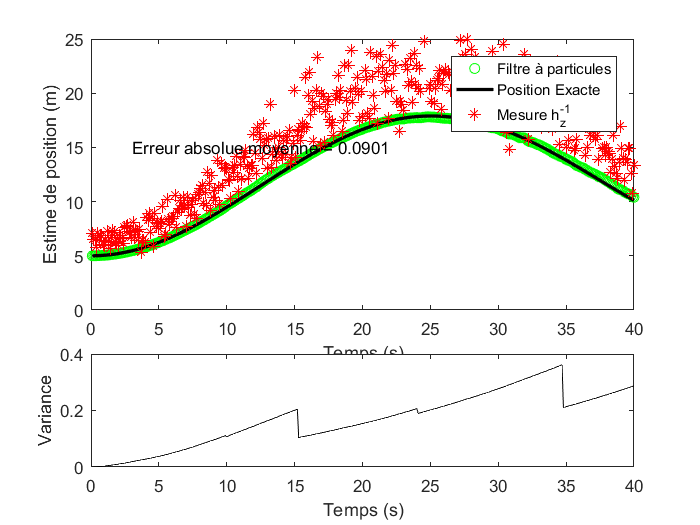
\includegraphics[width=1.0\textwidth]{fp1.png} 
  \end{tabular}
 \end{center}
 \vspace{-0.3in}
 \caption{Filtre à particules cas a, C = 40}
 \label{FP1}
\end{figure}

\noindent b) $X \in [3, 12]$ \\

\begin{table}[!ht]
\centering
\begin{tabular}{| c | c | c | c |}
 \hline
  C            &    4      &   10   &   40  \\ 
 \hline
  Précision    &  0.0641   & 0.0580 & 0.2273 \\ 
 \hline
\end{tabular}
\caption{Comparaison cas b}
\label{tab:FilterParticle1}
\end{table}

\vspace{-0.3in}
\label{FP}
\begin{figure}[ht]
 \begin{center}
  \begin{tabular}{c}
    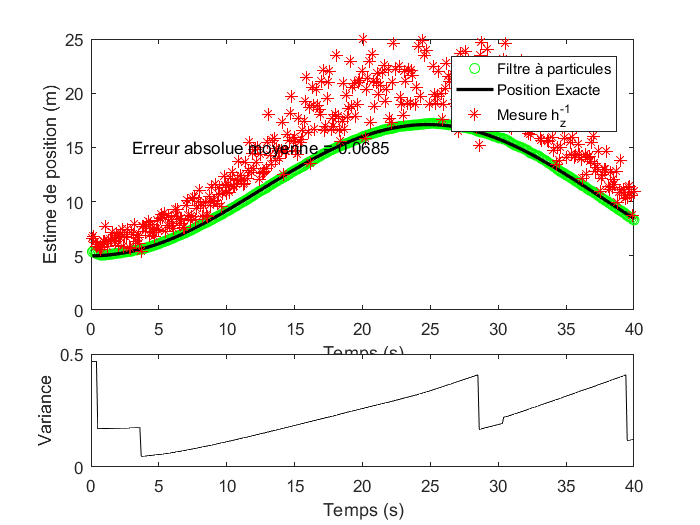
\includegraphics[width=1.0\textwidth]{fp2.png} 
  \end{tabular}
 \end{center}
 \vspace{-0.3in}
 \caption{Filtre à particules cas b, C = 40}
 \label{FP2}
\end{figure}

% =========================   E K F  ========================= 
\newpage
\section{Solution par filtre Kalman étendu (EKF)}
\label{EKF}
\subsection{Matrices $\Phi$, $\Gamma$, et $\Lambda$}

\noindent $\Phi = \begin{bmatrix}1 & dT\\0 & 1\end{bmatrix}$ \\

\noindent $\Gamma = \begin{bmatrix}dT^2/2 & dT\end{bmatrix}^T$ \\

\noindent $\Lambda = \begin{bmatrix}-(1/8.0)*Pwifi*exp(-X(1,1)/8.0) & 0\end{bmatrix}$ \\

\subsection{Implémentation du filtre EKF}

\noindent a) $X=[d_{init} \mbox{ }0]^T$, $P=\begin{bmatrix}0 &0\\0 & 0\end{bmatrix}$ \\ \\ \\  \\  \\

\vspace{-0.3in}
\label{EKF}
\begin{figure}[ht]
 \begin{center}
  \begin{tabular}{c}
    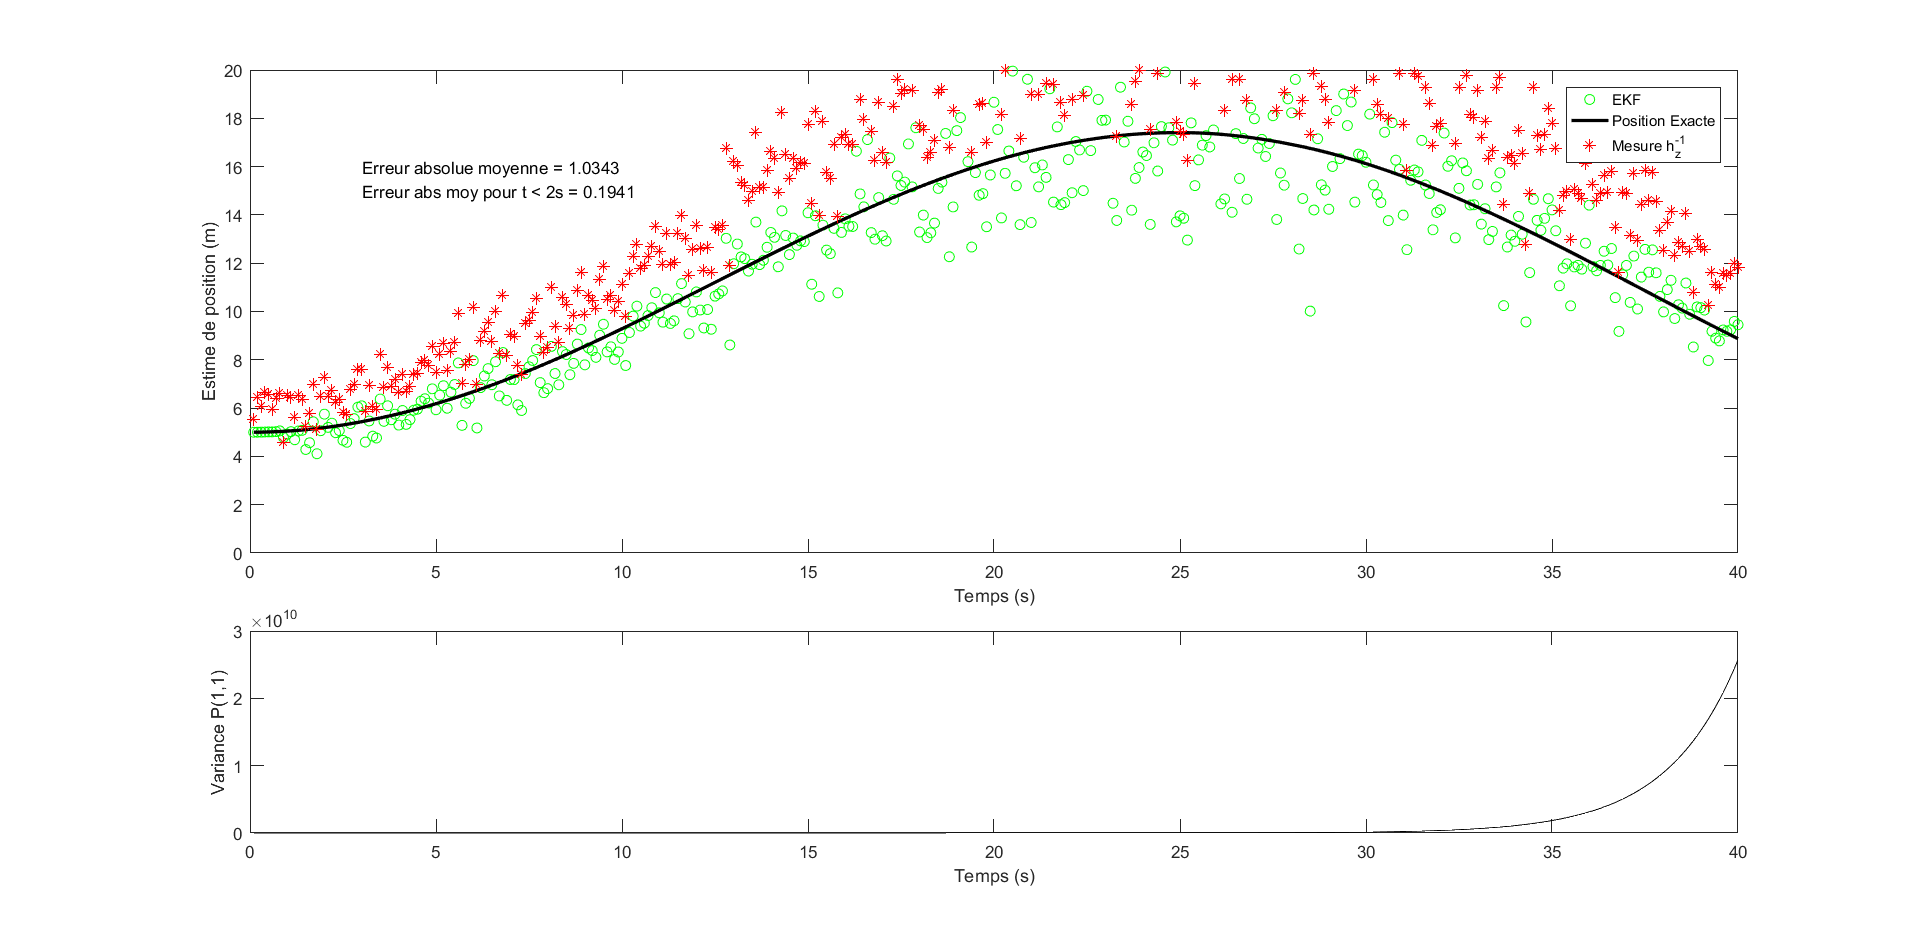
\includegraphics[width=1.0\textwidth]{ekf1.png} 
  \end{tabular}
 \end{center}
 \vspace{-0.3in}
 \caption{EKF 1}
 \label{EKF1}
\end{figure}

\noindent b) $X = [d_{init}\; 0]^T$ et $P = \begin{bmatrix}25 & 0\\0 & 0\end{bmatrix}$\\ \\ \\

\vspace{-0.3in}
\label{EKF}
\begin{figure}[ht]
 \begin{center}
  \begin{tabular}{c}
    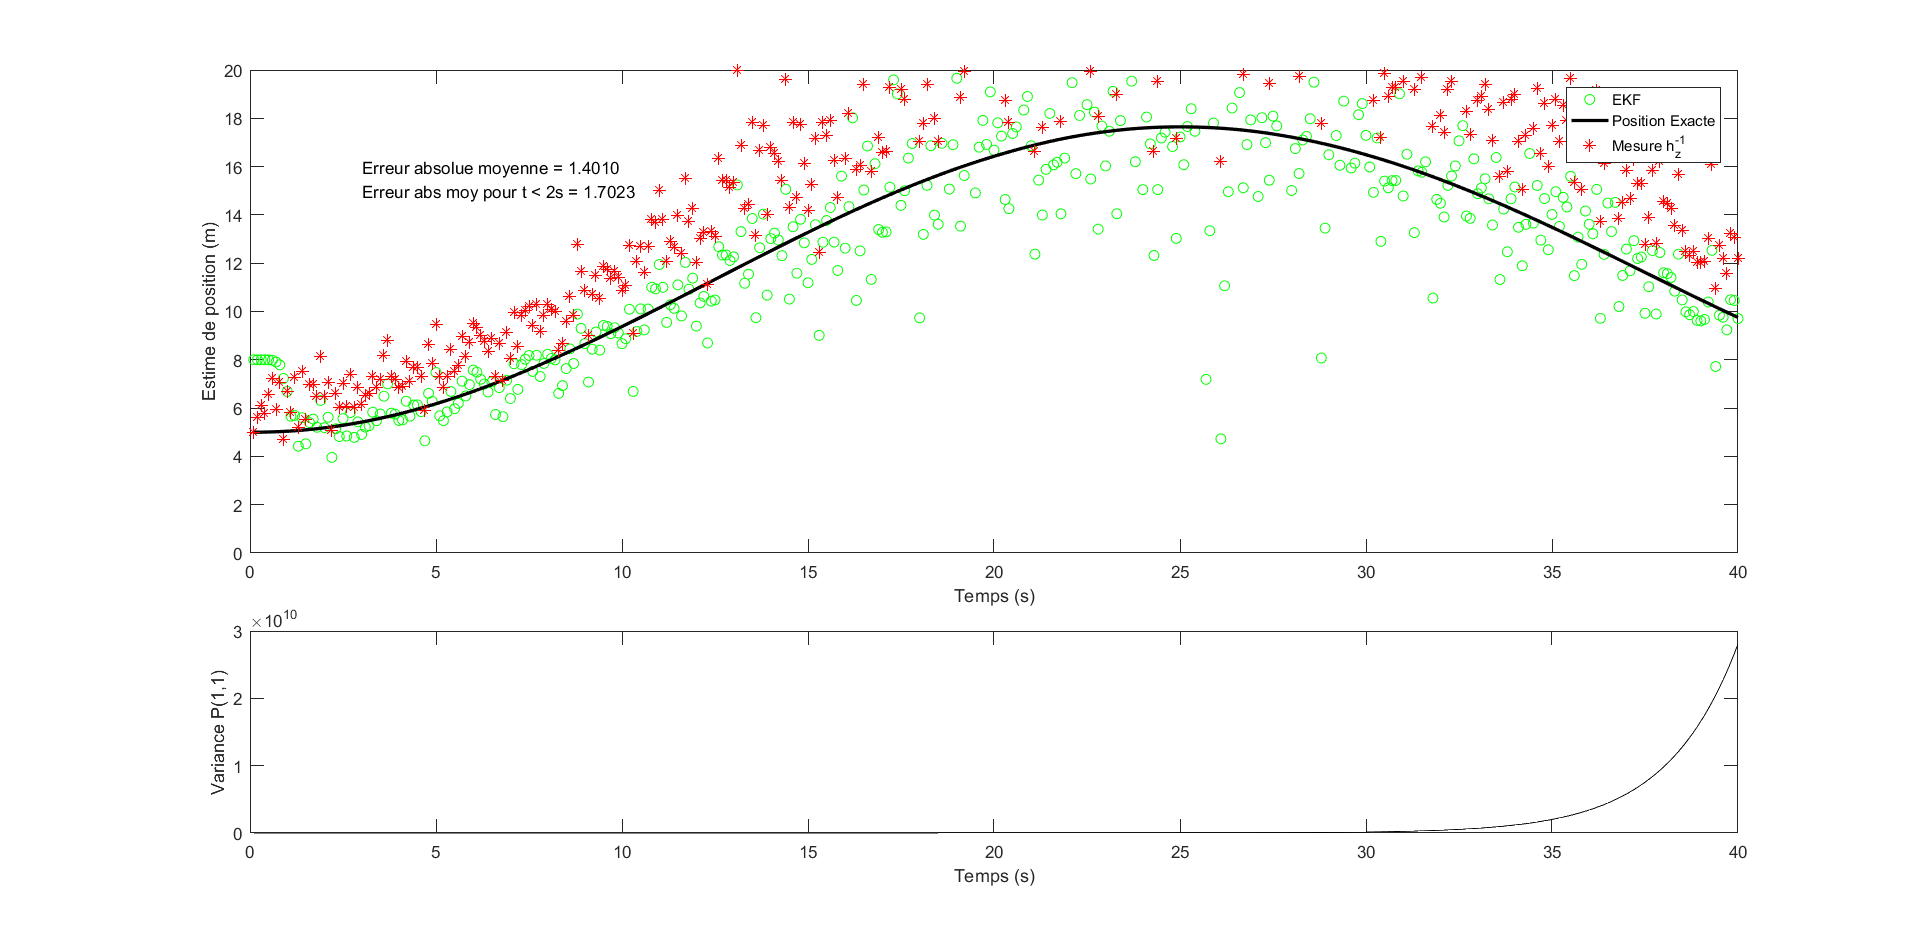
\includegraphics[width=1.0\textwidth]{ekf2.png} 
  \end{tabular}
 \end{center}
 \vspace{-0.3in}
 \caption{EKF 2}
 \label{EKF}
\end{figure}

\noindent c) $X = [8\; 0]^T$ et $P = \begin{bmatrix}0 & 0\\0 & 0\end{bmatrix}$ \\ \\ \\ \\ \\

\vspace{-0.3in}
\label{EKF}
\begin{figure}[ht]
 \begin{center}
  \begin{tabular}{c}
    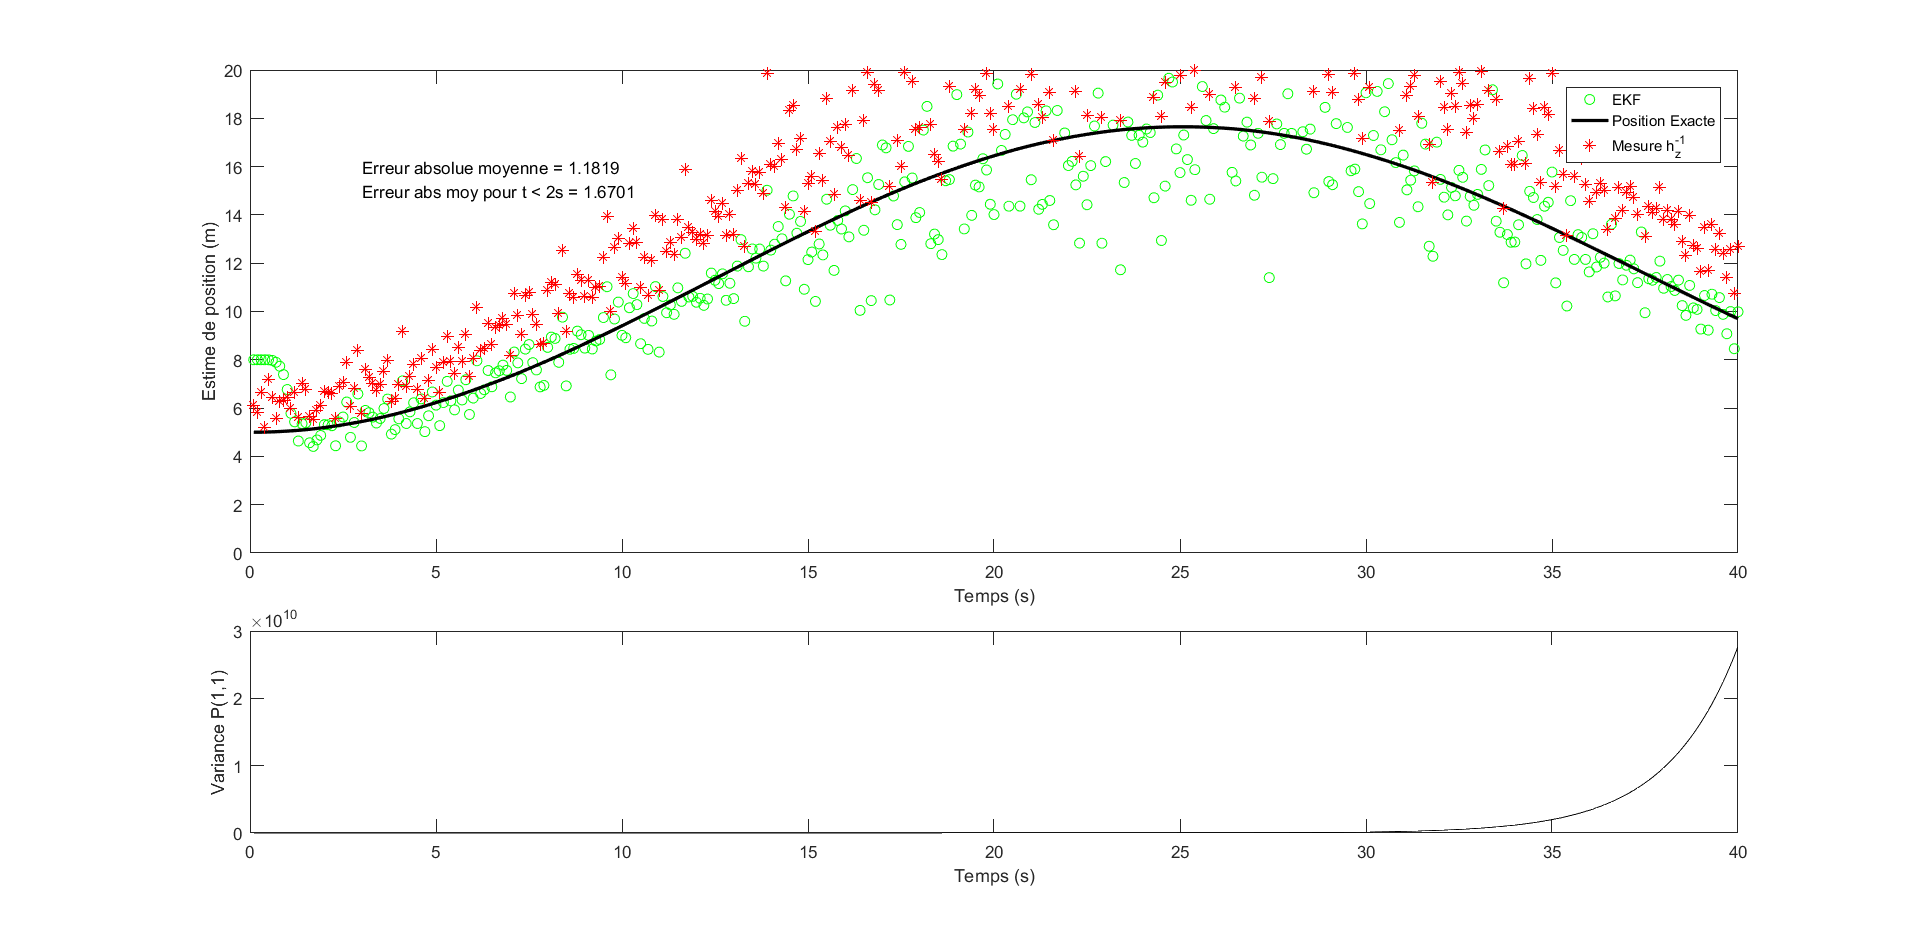
\includegraphics[width=1.0\textwidth]{ekf3.png} 
  \end{tabular}
 \end{center}
 \vspace{-0.3in}
 \caption{EKF3}
 \label{EKF3}
\end{figure}

\noindent d) $X = [8\; 0]^T$ et $P = \begin{bmatrix}100 & 0\\0 & 1\end{bmatrix}$ \\ \\ \\

\vspace{-0.3in}
\label{EKF}
\begin{figure}[ht]
 \begin{center}
  \begin{tabular}{c}
    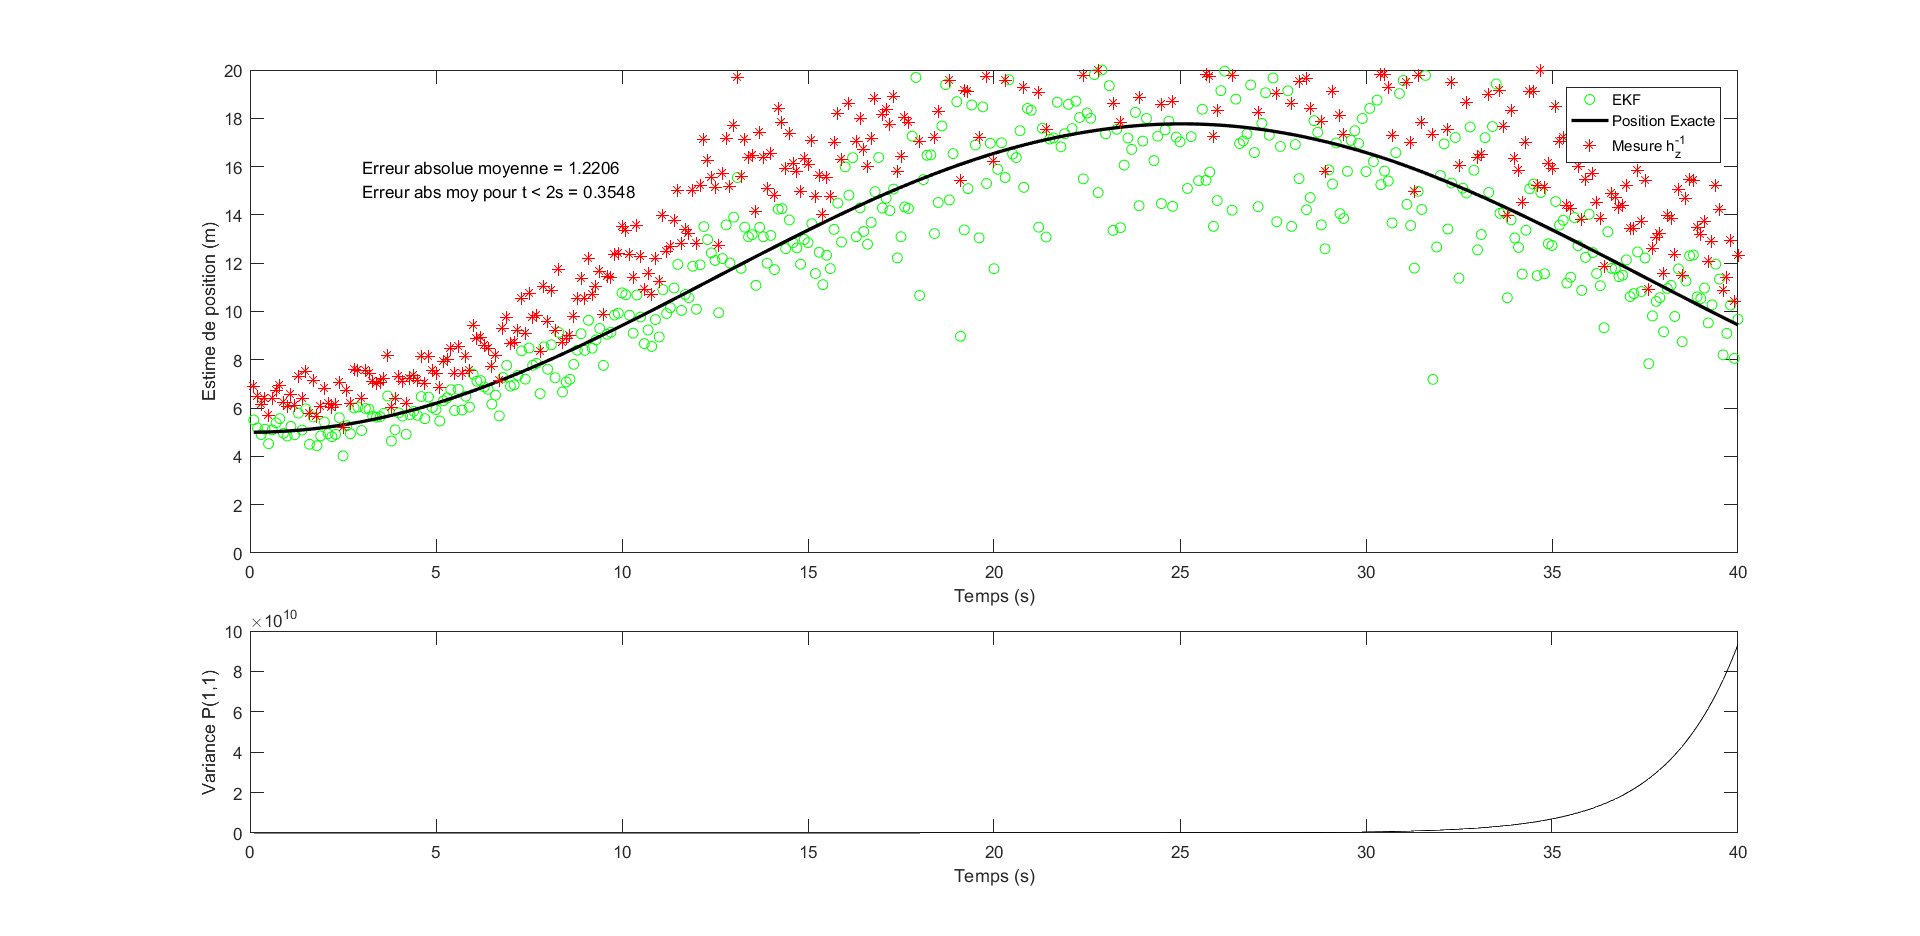
\includegraphics[width=0.95\textwidth]{ekf4.png} 
  \end{tabular}
 \end{center}
 \vspace{-0.3in}
 \caption{EKF4}
 \label{EKF4}
\end{figure}

\noindent Dans tous les cas a, b, c et d ci-dessus, notre algorithme parvient à converger rapidement et retrouver la position réelle du chariot. \\

\noindent Dans la situation a, on part de la position initiale réelle avec une totale confiance sur l'estimé de notre position. Notre EKF donne donc plus de crédit à notre estimé qu'au capteur et tout va bien car on avait bon. \\

\noindent Dans la situation b, on part avec une valeur initiale correcte sur la position du chariot mais, on n'est pas totalement certain de notre estimé. Cela nous prend quelques itérations, mais on finit par converger et retrouver la pose réelle du chariot. \\

\noindent Dans la situation c, on part avec une valeur initiale biaisée sur la position du chariot et une confiance totale en notre estimé. Le biais sur la position étant faible, on parvient quand même après quelques itérations à retrouver une bonne approximation de notre position réelle.  \\

\noindent Dans la situation d, on part avec une valeur initiale biaisée sur la position du chariot mais on fait plus confiance en notre capteur. Donc l'algorithme parvient à converger dès la première itération. 

\subsection{Divergence du filtre EKF}

\vspace{-0.3in}
\label{EKF}
\begin{figure}[ht]
 \begin{center}
  \begin{tabular}{c}
    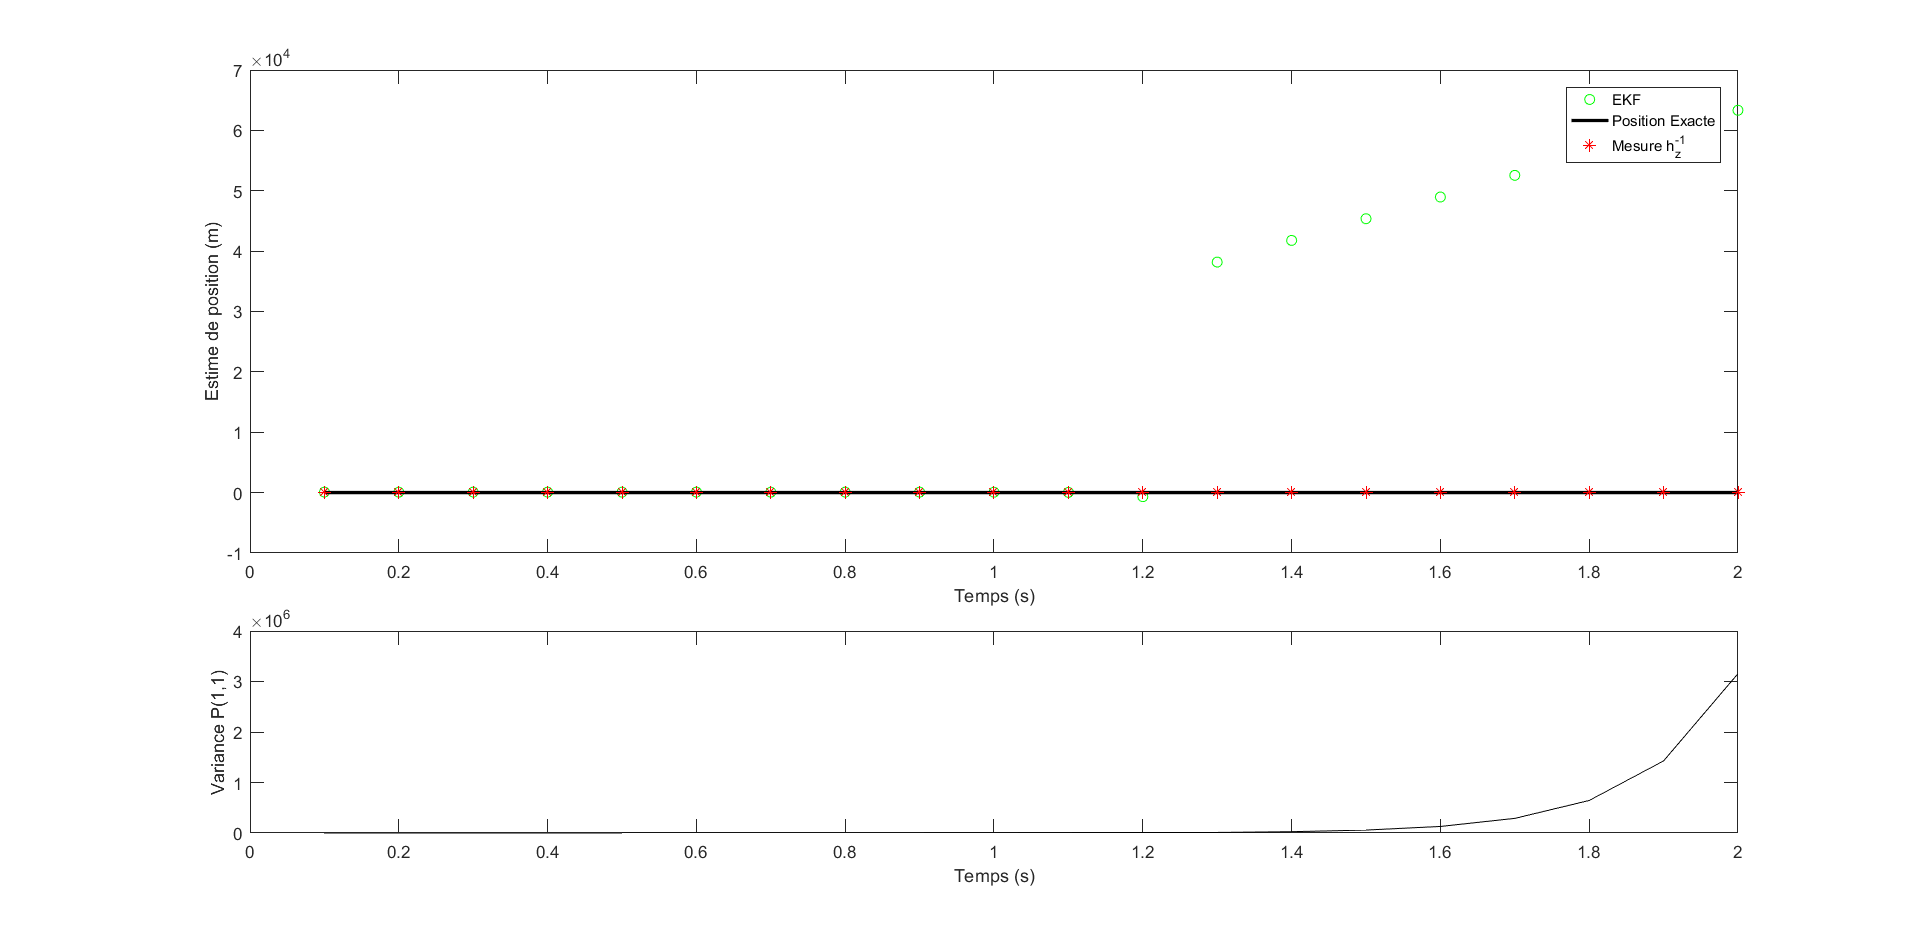
\includegraphics[width=1.0\textwidth]{ekf_div.png} 
  \end{tabular}
 \end{center}
 \vspace{-0.3in}
 \caption{EKF5}
 \label{EKF5}
\end{figure}

La distance initiale déterminée est $X = [80\; 0]^T$ et la matrice de covariance est $P = \begin{bmatrix}0 & 0\\0 & 3\end{bmatrix}$


% ===== L o c a l i s a t i o n   G l o b a l e -- F i l t r e   à   p a r t i c u l e s   =====
\newpage
\section {Localisation globale par filtre à particules}
\label{LocalisationGlobale}

\subsection{Cas 1 : l'angle est connu}
\label{Q1Global}

\noindent Discussion:

\noindent Etant donné qu'on ne connait pas la position du robot il nous faut avoir assez de particules pour l'approximer correctement. Ayant une grande surface, on a déterminé que 1000 particules est le plus petit nombre nécessaire pour converger le plus de fois. \\

\noindent Pour $S_V$ on décidé de surestimer sa valeur par rapport à la valeur réelle. On a donc fait des tests en incrémentant cette valeur de 0.01 à chaque fois. Et on a déterminé que celle qui donne les meilleurs résultats est 0.1. \\

\noindent On choisit $\sigma_{angle}$  pas trop grand pour empêcher de dévier de la position réelle de notre robot si on converge et également pas trop petit pour pouvoir brasser suffisament l'angle du robot et changer la tendance en cas de mauvais positionnement. 

\noindent Pour cela, on a fait plusieurs tests en icrémentant à chaque fois la valeur de $\sigma_{angle}$ de 0.01 à chaque fois on mesure l'erreur moyenne obtenue. Les résultats obtenus sont contenus dans le graphe suivant. \\ 

\vspace{0.3in}
\label{LFP}
\begin{figure}[ht]
 \begin{center}
  \begin{tabular}{c}
    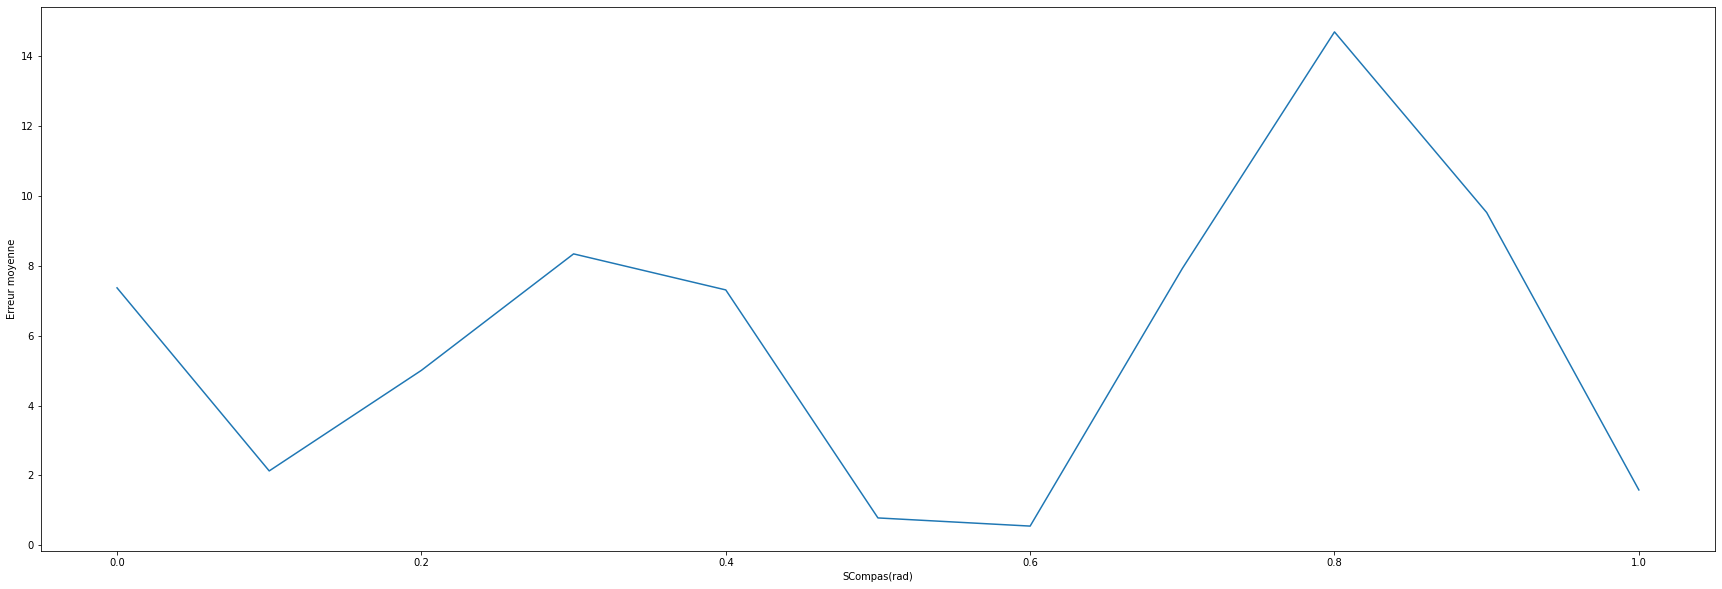
\includegraphics[width=1.0\textwidth]{lfp_scompas_err.png} 
  \end{tabular}
 \end{center}
 \vspace{-0.3in}
 \caption{Erreur moyenne en fonction de $\sigma_{angle}$}
 \label{LFP}
\end{figure}

\noindent On peut donc déterminer que la valeur de $\sigma_{angle}$ pour laquelle on obtient un score minimal est 0.6. \\

\noindent Les particules disposées uniformément sur la carte se concentrent rapidement autour de certains points. Et en quelques itérations il parvient à se rassembler autour d'un seul centre. \\

\vspace{0.3in}
\label{LFP}
\begin{figure}[ht]
 \begin{center}
  \begin{tabular}{c}
    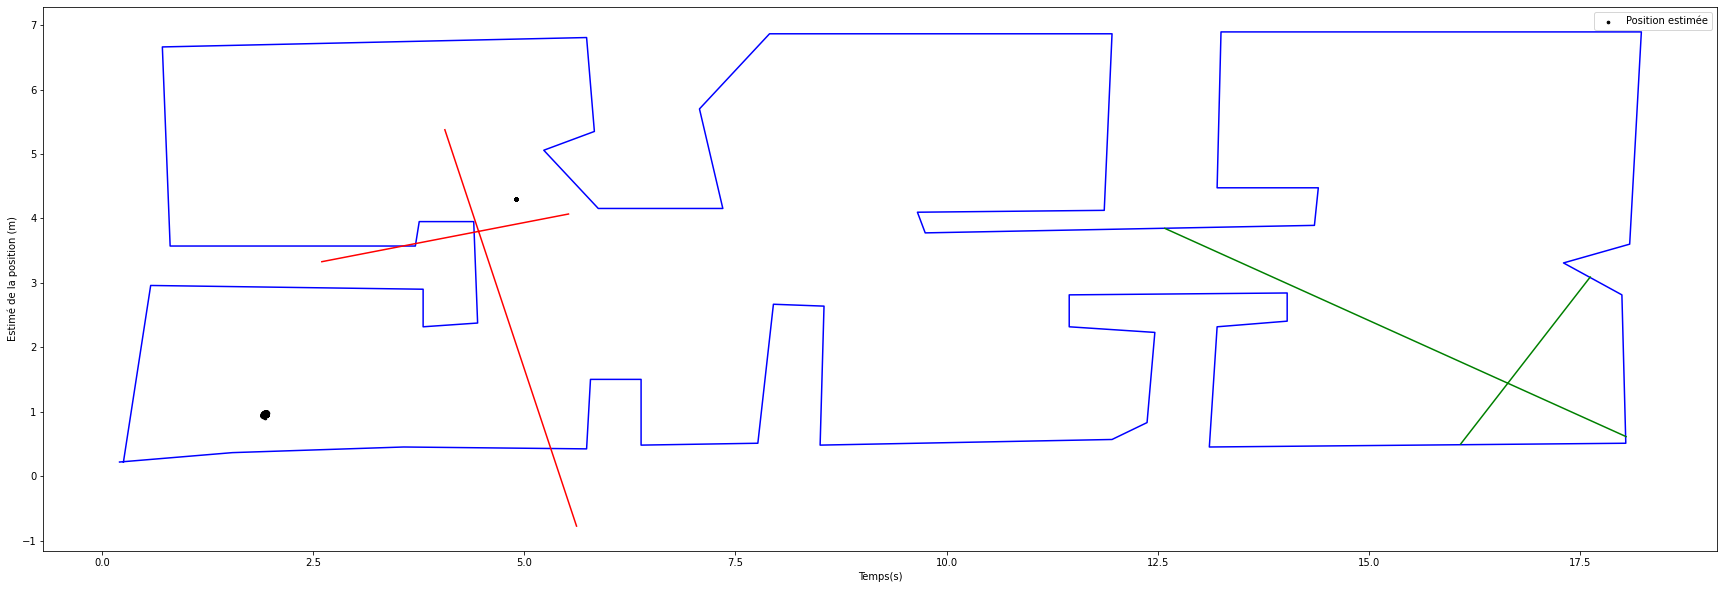
\includegraphics[width=1.0\textwidth]{lfp_err.png} 
  \end{tabular}
 \end{center}
 \vspace{-0.3in}
 \caption{Filtre à particules diverge}
 \label{LFP}
\end{figure}

\vspace{0.3in}
\label{LFP}
\begin{figure}[ht]
 \begin{center}
  \begin{tabular}{c}
    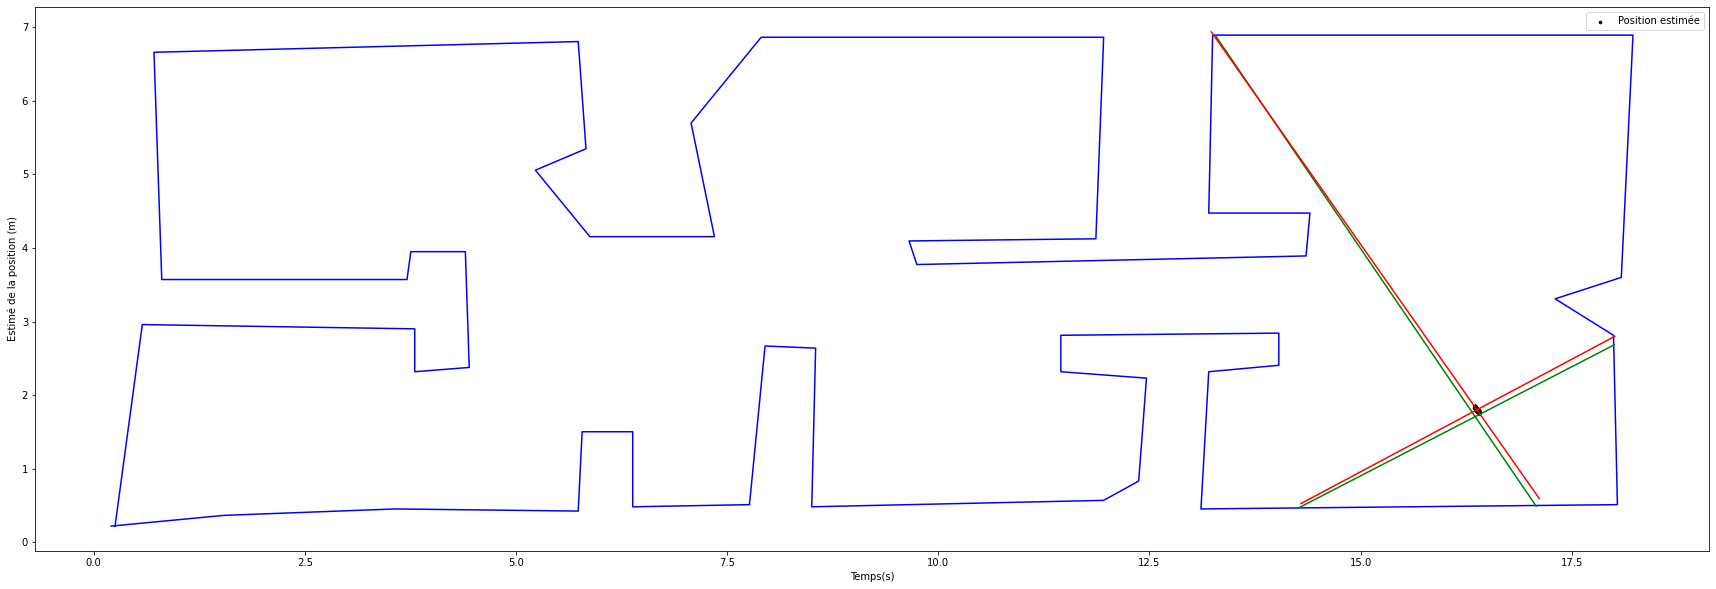
\includegraphics[width=1.0\textwidth]{lfp_success.png} 
  \end{tabular}
 \end{center}
 \vspace{-0.3in}
 \caption{Filtre à particules converge}
 \label{LFP}
\end{figure}

\noindent Le filtre peut échouer à cause de plusieurs raisons: 
\begin{itemize}
\item Une mauvaise configuration dès le départ des particules qui ne couvrent pas toutes la surface du polygone;
\item De plus, plusieurs zones de la carte se ressemblent et induisent donc facilement en erreur notre algorithme.
\end{itemize}

\newpage
\subsection{Impact du bruit utilisé dans la vraisemblance LiDAR}

\noindent On a fait plusieurs tests pour observer la comment se comporte l'erreur en fonction du choix de $\sigma_{LiDAR}$. On a constaté que plus $\sigma_{LiDAR}$ est petit, plus il faut de particules pour pouvoir converger. A contrario, plus $\sigma_{LiDAR}$ est grand et moins vite il converge. \\

\noindent Le graphe ci-dessous montre l'erreur moyenne en fonction du choix de $\sigma_{LiDAR}$. On peut remarquer grâce à celui-ci que plus $\sigma_{LiDAR}$ est grand plus l'erreur est grande. Cela montre qu'on tolère plus d'estimations grossières. On pourrait cependant réussir à obtenir de bon résultat par chance lorsque les particules sont bien placées dès le départ. C'est ce qui explique le pic inversé pour $\sigma_{LiDAR} = 0.7$. 

\vspace{0.3in}
\label{LFP}
\begin{figure}[ht]
 \begin{center}
  \begin{tabular}{c}
    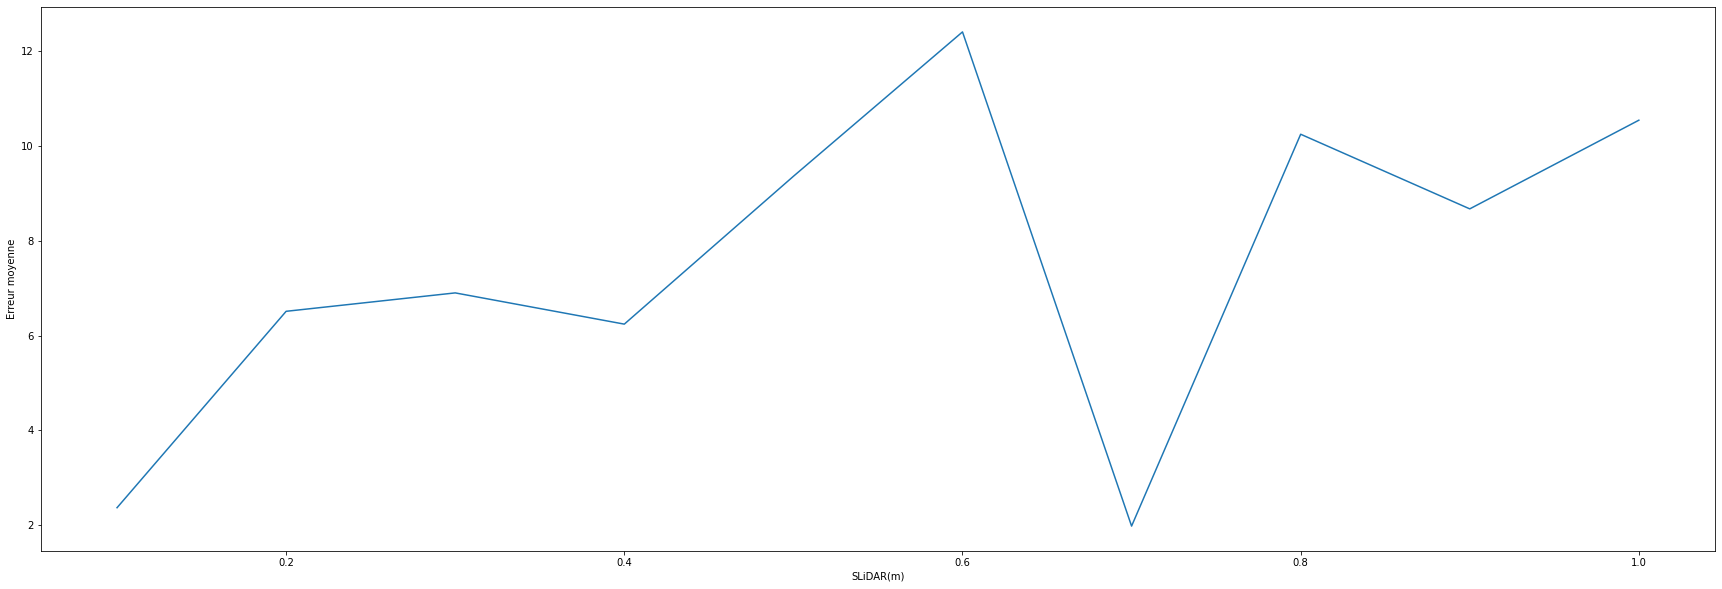
\includegraphics[width=1.0\textwidth]{lfp_slidar_err.png} 
  \end{tabular}
 \end{center}
 \vspace{-0.3in}
 \caption{Erreur moyenne en fonction de $\sigma_{LiDAR}$}
 \label{LFP}
\end{figure}

\newpage
\noindent Il serait donc intéressant d'augmenter la valeur de $\sigma_{LiDAR}$ au fil du temps pour éviter à notre algorithme de sauter aux conclusions rapidement lorsqu'on tombe sur des coins similaires à notre position réelle. 

\end{document}
